% Created by tikzDevice version 0.7.0 on 2014-04-27 13:00:04
% !TEX encoding = UTF-8 Unicode
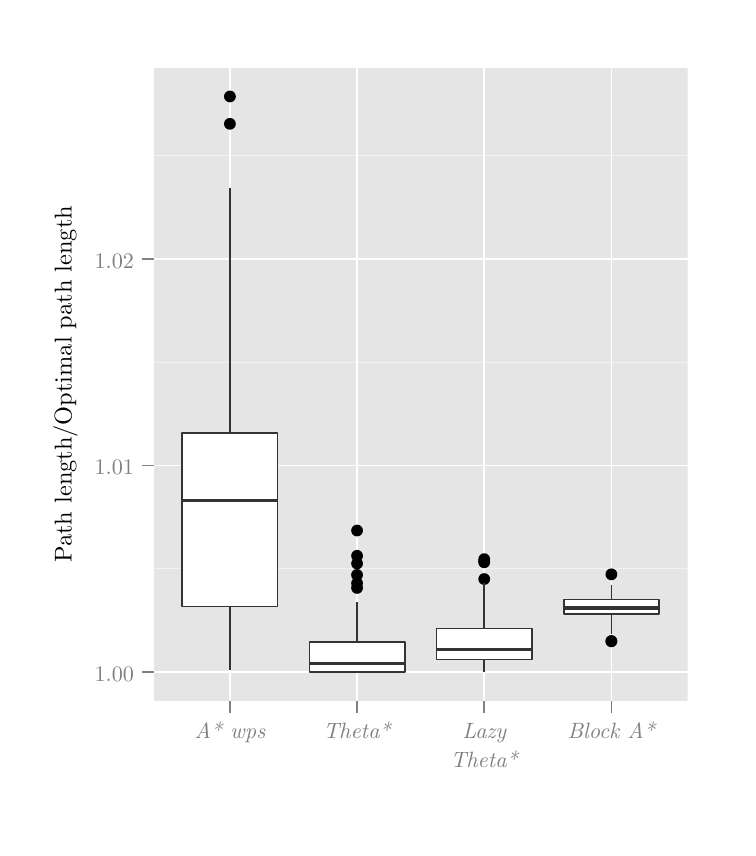
\begin{tikzpicture}[x=1pt,y=1pt]
\definecolor[named]{fillColor}{rgb}{1.00,1.00,1.00}
\path[use as bounding box,fill=fillColor,fill opacity=0.00] (0,0) rectangle (252.94,289.08);
\begin{scope}
\path[clip] (  0.00,  0.00) rectangle (252.94,289.08);
\definecolor[named]{drawColor}{rgb}{1.00,1.00,1.00}
\definecolor[named]{fillColor}{rgb}{1.00,1.00,1.00}

\path[draw=drawColor,line width= 0.6pt,line join=round,line cap=round,fill=fillColor] (  0.00, -0.00) rectangle (252.94,289.08);
\end{scope}
\begin{scope}
\path[clip] ( 45.51, 45.78) rectangle (238.49,274.63);
\definecolor[named]{fillColor}{rgb}{0.90,0.90,0.90}

\path[fill=fillColor] ( 45.51, 45.78) rectangle (238.49,274.63);
\definecolor[named]{drawColor}{rgb}{0.95,0.95,0.95}

\path[draw=drawColor,line width= 0.3pt,line join=round] ( 45.51, 93.51) --
	(238.49, 93.51);

\path[draw=drawColor,line width= 0.3pt,line join=round] ( 45.51,168.16) --
	(238.49,168.16);

\path[draw=drawColor,line width= 0.3pt,line join=round] ( 45.51,242.81) --
	(238.49,242.81);
\definecolor[named]{drawColor}{rgb}{1.00,1.00,1.00}

\path[draw=drawColor,line width= 0.6pt,line join=round] ( 45.51, 56.18) --
	(238.49, 56.18);

\path[draw=drawColor,line width= 0.6pt,line join=round] ( 45.51,130.83) --
	(238.49,130.83);

\path[draw=drawColor,line width= 0.6pt,line join=round] ( 45.51,205.48) --
	(238.49,205.48);

\path[draw=drawColor,line width= 0.6pt,line join=round] ( 73.08, 45.78) --
	( 73.08,274.63);

\path[draw=drawColor,line width= 0.6pt,line join=round] (119.02, 45.78) --
	(119.02,274.63);

\path[draw=drawColor,line width= 0.6pt,line join=round] (164.97, 45.78) --
	(164.97,274.63);

\path[draw=drawColor,line width= 0.6pt,line join=round] (210.92, 45.78) --
	(210.92,274.63);
\definecolor[named]{fillColor}{rgb}{0.00,0.00,0.00}

\path[fill=fillColor] ( 73.08,264.22) circle (  2.13);

\path[fill=fillColor] ( 73.08,254.33) circle (  2.13);
\definecolor[named]{drawColor}{rgb}{0.20,0.20,0.20}
\definecolor[named]{fillColor}{rgb}{0.20,0.20,0.20}

\path[draw=drawColor,line width= 0.6pt,line join=round,fill=fillColor] ( 73.08,142.59) -- ( 73.08,231.28);

\path[draw=drawColor,line width= 0.6pt,line join=round,fill=fillColor] ( 73.08, 79.93) -- ( 73.08, 56.89);
\definecolor[named]{fillColor}{rgb}{1.00,1.00,1.00}

\path[draw=drawColor,line width= 0.6pt,line join=round,line cap=round,fill=fillColor] ( 55.84,142.59) --
	( 55.84, 79.93) --
	( 90.31, 79.93) --
	( 90.31,142.59) --
	( 55.84,142.59) --
	cycle;
\definecolor[named]{fillColor}{rgb}{0.20,0.20,0.20}

\path[draw=drawColor,line width= 1.1pt,line join=round,fill=fillColor] ( 55.84,118.28) -- ( 90.31,118.28);
\definecolor[named]{fillColor}{rgb}{0.00,0.00,0.00}

\path[fill=fillColor] (119.02,107.37) circle (  2.13);

\path[fill=fillColor] (119.02, 98.24) circle (  2.13);

\path[fill=fillColor] (119.02, 86.63) circle (  2.13);

\path[fill=fillColor] (119.02, 91.33) circle (  2.13);

\path[fill=fillColor] (119.02, 95.44) circle (  2.13);

\path[fill=fillColor] (119.02, 88.33) circle (  2.13);
\definecolor[named]{fillColor}{rgb}{0.20,0.20,0.20}

\path[draw=drawColor,line width= 0.6pt,line join=round,fill=fillColor] (119.02, 67.18) -- (119.02, 81.46);

\path[draw=drawColor,line width= 0.6pt,line join=round,fill=fillColor] (119.02, 56.28) -- (119.02, 56.18);
\definecolor[named]{fillColor}{rgb}{1.00,1.00,1.00}

\path[draw=drawColor,line width= 0.6pt,line join=round,line cap=round,fill=fillColor] (101.79, 67.18) --
	(101.79, 56.28) --
	(136.25, 56.28) --
	(136.25, 67.18) --
	(101.79, 67.18) --
	cycle;
\definecolor[named]{fillColor}{rgb}{0.20,0.20,0.20}

\path[draw=drawColor,line width= 1.1pt,line join=round,fill=fillColor] (101.79, 59.19) -- (136.25, 59.19);
\definecolor[named]{fillColor}{rgb}{0.00,0.00,0.00}

\path[fill=fillColor] (164.97, 97.03) circle (  2.13);

\path[fill=fillColor] (164.97, 89.84) circle (  2.13);

\path[fill=fillColor] (164.97, 95.89) circle (  2.13);

\path[fill=fillColor] (164.97, 96.23) circle (  2.13);
\definecolor[named]{fillColor}{rgb}{0.20,0.20,0.20}

\path[draw=drawColor,line width= 0.6pt,line join=round,fill=fillColor] (164.97, 71.95) -- (164.97, 88.58);

\path[draw=drawColor,line width= 0.6pt,line join=round,fill=fillColor] (164.97, 60.75) -- (164.97, 56.18);
\definecolor[named]{fillColor}{rgb}{1.00,1.00,1.00}

\path[draw=drawColor,line width= 0.6pt,line join=round,line cap=round,fill=fillColor] (147.74, 71.95) --
	(147.74, 60.75) --
	(182.20, 60.75) --
	(182.20, 71.95) --
	(147.74, 71.95) --
	cycle;
\definecolor[named]{fillColor}{rgb}{0.20,0.20,0.20}

\path[draw=drawColor,line width= 1.1pt,line join=round,fill=fillColor] (147.74, 64.35) -- (182.20, 64.35);
\definecolor[named]{fillColor}{rgb}{0.00,0.00,0.00}

\path[fill=fillColor] (210.92, 91.54) circle (  2.13);

\path[fill=fillColor] (210.92, 67.35) circle (  2.13);

\path[fill=fillColor] (210.92, 67.43) circle (  2.13);
\definecolor[named]{fillColor}{rgb}{0.20,0.20,0.20}

\path[draw=drawColor,line width= 0.6pt,line join=round,fill=fillColor] (210.92, 82.47) -- (210.92, 87.85);

\path[draw=drawColor,line width= 0.6pt,line join=round,fill=fillColor] (210.92, 77.10) -- (210.92, 69.95);
\definecolor[named]{fillColor}{rgb}{1.00,1.00,1.00}

\path[draw=drawColor,line width= 0.6pt,line join=round,line cap=round,fill=fillColor] (193.69, 82.47) --
	(193.69, 77.10) --
	(228.15, 77.10) --
	(228.15, 82.47) --
	(193.69, 82.47) --
	cycle;
\definecolor[named]{fillColor}{rgb}{0.20,0.20,0.20}

\path[draw=drawColor,line width= 1.1pt,line join=round,fill=fillColor] (193.69, 79.37) -- (228.15, 79.37);
\end{scope}
\begin{scope}
\path[clip] (  0.00,  0.00) rectangle (252.94,289.08);
\definecolor[named]{drawColor}{rgb}{0.50,0.50,0.50}

\node[text=drawColor,anchor=base east,inner sep=0pt, outer sep=0pt, scale=  0.80] at ( 38.39, 52.87) {1.00};

\node[text=drawColor,anchor=base east,inner sep=0pt, outer sep=0pt, scale=  0.80] at ( 38.39,127.53) {1.01};

\node[text=drawColor,anchor=base east,inner sep=0pt, outer sep=0pt, scale=  0.80] at ( 38.39,202.18) {1.02};
\end{scope}
\begin{scope}
\path[clip] (  0.00,  0.00) rectangle (252.94,289.08);
\definecolor[named]{drawColor}{rgb}{0.50,0.50,0.50}

\path[draw=drawColor,line width= 0.6pt,line join=round] ( 41.24, 56.18) --
	( 45.51, 56.18);

\path[draw=drawColor,line width= 0.6pt,line join=round] ( 41.24,130.83) --
	( 45.51,130.83);

\path[draw=drawColor,line width= 0.6pt,line join=round] ( 41.24,205.48) --
	( 45.51,205.48);
\end{scope}
\begin{scope}
\path[clip] (  0.00,  0.00) rectangle (252.94,289.08);
\definecolor[named]{drawColor}{rgb}{0.50,0.50,0.50}

\path[draw=drawColor,line width= 0.6pt,line join=round] ( 73.08, 41.51) --
	( 73.08, 45.78);

\path[draw=drawColor,line width= 0.6pt,line join=round] (119.02, 41.51) --
	(119.02, 45.78);

\path[draw=drawColor,line width= 0.6pt,line join=round] (164.97, 41.51) --
	(164.97, 45.78);

\path[draw=drawColor,line width= 0.6pt,line join=round] (210.92, 41.51) --
	(210.92, 45.78);
\end{scope}
\begin{scope}
\path[clip] (  0.00,  0.00) rectangle (252.94,289.08);
\definecolor[named]{drawColor}{rgb}{0.50,0.50,0.50}

\node[text=drawColor,anchor=base,inner sep=0pt, outer sep=0pt, scale=  0.80] at ( 73.08, 32.05) {{\em A* wps}};

\node[text=drawColor,anchor=base,inner sep=0pt, outer sep=0pt, scale=  0.80] at (119.02, 32.05) {{\em Theta*}};

\node[text=drawColor,anchor=base,inner sep=0pt, outer sep=0pt, scale=  0.80] at (164.97, 32.05) {{\em Lazy}};

\node[text=drawColor,anchor=base,inner sep=0pt, outer sep=0pt, scale=  0.80] at (164.97, 21.69) {{\em Theta*}};

\node[text=drawColor,anchor=base,inner sep=0pt, outer sep=0pt, scale=  0.80] at (210.92, 32.05) {{\em Block A*}};
\end{scope}
\begin{scope}
\path[clip] (  0.00,  0.00) rectangle (252.94,289.08);
\definecolor[named]{drawColor}{rgb}{0.00,0.00,0.00}

\node[text=drawColor,rotate= 90.00,anchor=base,inner sep=0pt, outer sep=0pt, scale=  0.88] at ( 15.90,160.20) {Path length/Optimal path length};
\end{scope}
\end{tikzpicture}
